%% example text content
%% scrartcl and scrreprt starts with section, subsection, subsubsection, ...
%% scrbook starts with part (optional), chapter, section, ...
\chapter{Securing an Example Application}

In this chapter, the security concepts introduced above are put into practice by applying them to a real-world application. This application has been created solely for demonstration purposes to resemble a typical use case while still retaining simplicity to be generally applicable and easy to understand.

\section{Example Application}

\paragraph{Functionality}

The example application is a simple dashboard for Kubernetes to view Pods in certain or all namespaces. It can also display ReplicaSets and scale them up by demand. A screenshot of it is depicted in Figure \ref{fig:exaScreenshot}.

\begin{figure}[H]
\begin{center}
    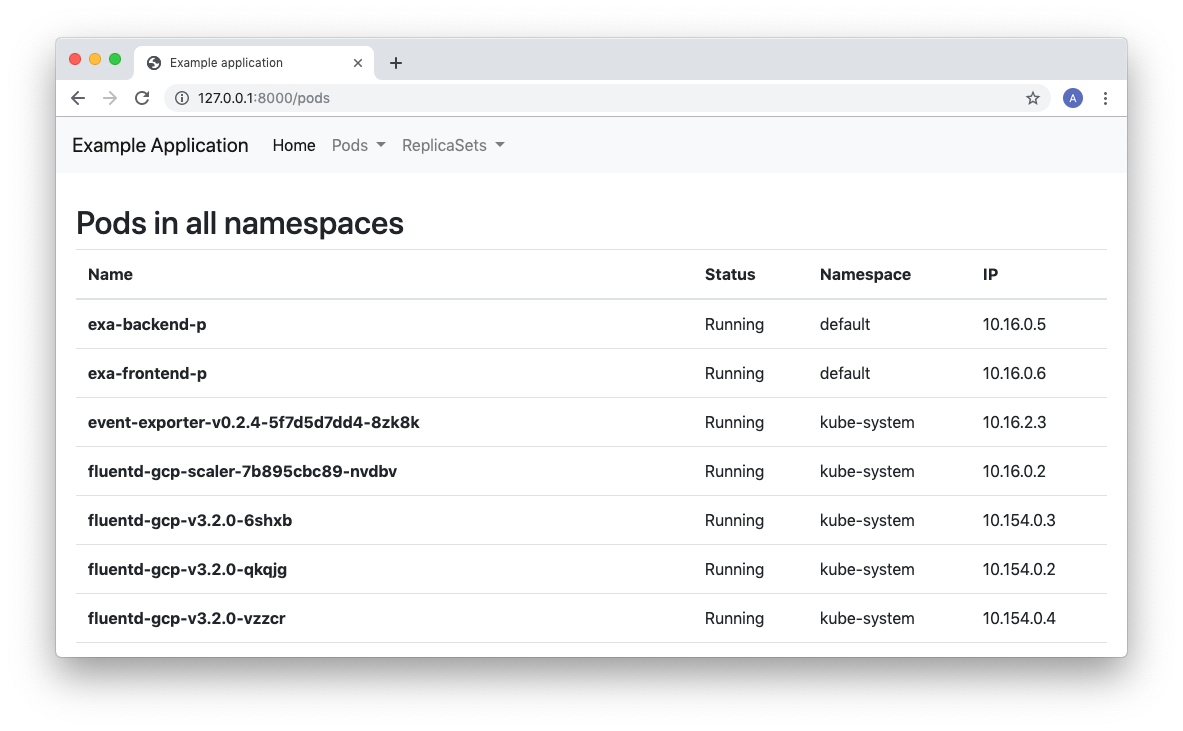
\includegraphics[width=1.0\linewidth]{figures/exa_screenshot.png}
    \caption[Screenshot of the example application]{This screenshot depicts the example application being port-forwarded to a local machine.}
    \label{fig:exaScreenshot}
\end{center}
\end{figure}

\paragraph{Setup}

The application is written in Python and makes use of Flask\footnote{\url{http://flask.pocoo.org/}, accessed 2019-07-02} as well as the Kubernetes Python Client\footnote{\url{https://github.com/kubernetes-client/python}, accessed 2019-07-02}. 

The setup consists of a backend \mycode{exa-backend} part and a frontend part \mycode{exa-frontend}. \mycode{exa-backend} provides a REST API with direct accesses to the Kubernetes API, while \mycode{exa-frontend} uses the backend for displaying the data. 

\begin{figure}[H]
\begin{center}
    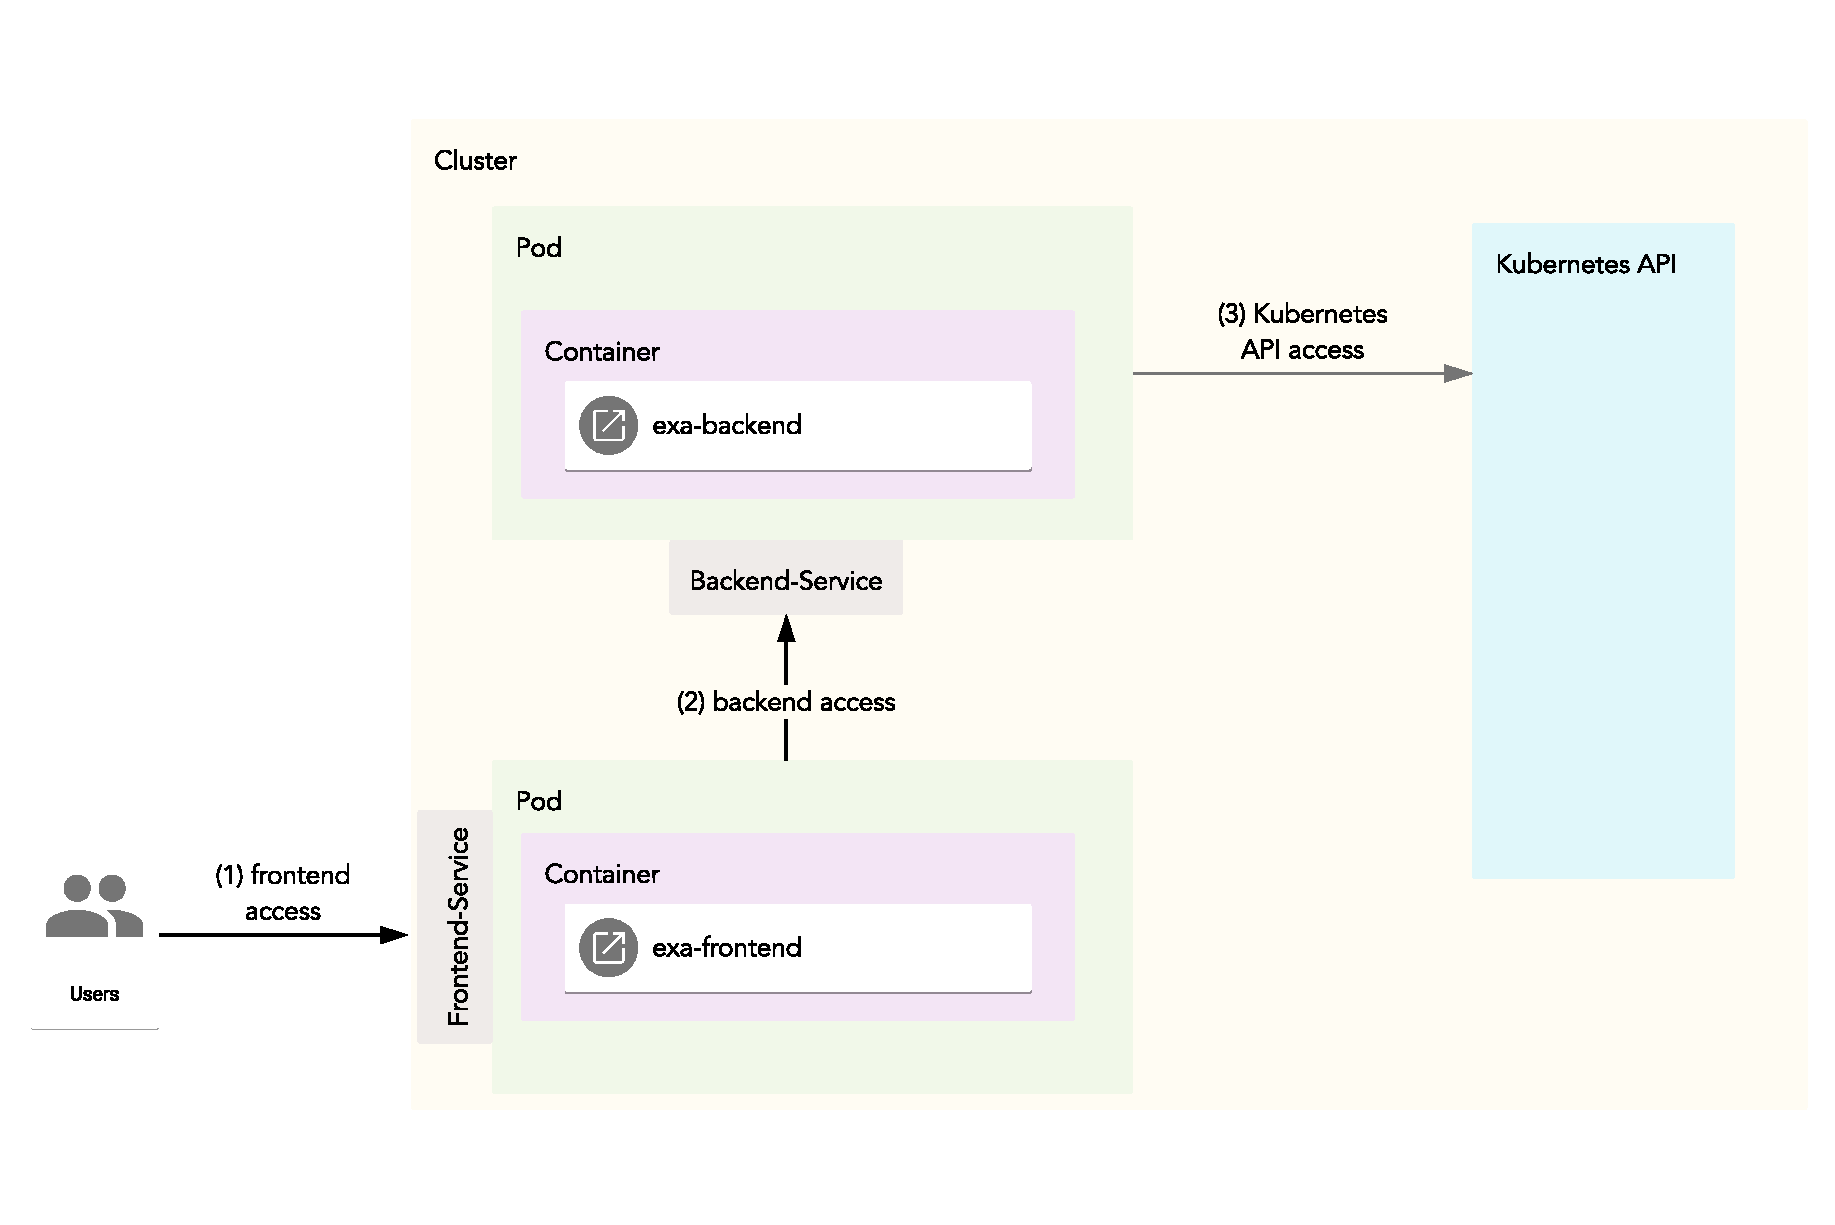
\includegraphics[width=1.0\linewidth]{figures/exa_architecture.pdf}
    \caption[Architecture of the example application]{This architecture diagram shows how the example application runs within the Kubernetes cluster.}
    \label{fig:exaArchitecture}
\end{center}
\end{figure}

The Kubernetes cluster is set up using \ac{GKE} on \ac{GCP}\footnote{\url{https://cloud.google.com/kubernetes-engine/}, accessed 2019-07-02}. It is a sensible choice for cluster administrators who are not yet experts in the field of Kubernetes security, as it scales well from a very basic setup up to a large high-availability cluster.

The architecture of the cluster is depicted in Figure~\ref{fig:exaArchitecture}. The frontend and backend components run in separate pods. Users access the frontend via an ingress that maps to the frontend service. The frontend then retrieves all information by calling the backend service, which in turn makes the request to the Kubernetes API to perform the user's query.

\section{Security Measures}

In this section, the measures that were taken to secure the setup are explained. They are structured according to the layer model introduced in Chapter~\ref{chap:clusterSecurity}.

\subsection{Base Infrastructure Security}

As this setup uses \ac{GKE} as an infrastructure provider, most considerations for base infrastructure security are already taken care of by Google\footnote{\url{https://cloud.google.com/kubernetes-engine/docs/concepts/security-overview}, accessed 2019-07-09}. By default, \ac{GKE} clusters run the newest version of Google's Container-Optimized OS\footnote{\url{https://cloud.google.com/container-optimized-os/docs/concepts/features-and-benefits}, accessed 2019-07-09} that comes with a current version of the container runtime as well. 

However, as all cluster components are running within the \ac{GCP} environment, they are also subject to Google's Cloud \ac{IAM}\footnote{\url{https://cloud.google.com/iam/}, accessed 2019-07-09}. It works alongside Kubernetes \ac{RBAC}, yet requires some special attention when applications within the Kubernetes cluster access other resources on \ac{GCP} outside of the cluster.\footnote{\url{https://cloud.google.com/kubernetes-engine/docs/how-to/iam}, accessed 2019-07-09}

\subsection{Kubernetes Infrastructure Security}

When it comes to Kubernetes' infrastructure components, most relevant security aspects are still closely tied to the underlying base infrastructure, in this case, \ac{GKE}.

\paragraph{API Server}

The aforementioned \ac{IAM}, by default, allows login using username and password. We disabled it in the cluster configuration in the \ac{GCP} web interface and only used certificates, which we regularly rotate\footnote{\url{https://cloud.google.com/kubernetes-engine/docs/how-to/credential-rotation}, accessed 2019-07-09}, to authenticate within the cluster.

\paragraph{Secret Encryption}

As explained in Section~\ref{ssec:etcd}, it is vital to encrypt all secrets stored in \mycode{etcd}. While \ac{GKE} uses encryption at rest by default\footnote{\url{https://cloud.google.com/security/encryption-at-rest/default-encryption/}, accessed 2019-07-09}, we also configured application-layer encryption in case an attacker gains access to an offline copy of the \mycode{etcd} database. To set up the encryption, we generated a key, stored it in Google's Cloud Key Management Service (KMS)\footnote{\url{https://cloud.google.com/kms/docs/}, accessed 2019-07-09} and handed it to the cluster configuration using \mycode{--database-encryption-key}\footnote{\url{https://cloud.google.com/kubernetes-engine/docs/how-to/encrypting-secrets}, accessed 2019-07-09}.  

\paragraph{Dashboard}

As the standard Kubernetes dashboard is deprecated and disabled by default on GKE, no further configuration was necessary to secure the setup. The \ac{GCP} Console\footnote{\url{https://console.cloud.google.com/}, accessed 2019-07-09}, which acts as a replacement for the standard dashboard on \ac{GKE}, again uses Google's \ac{IAM} and therefore needs no further protection. It is conceptually not accessible by unauthenticated users. 

\subsection{Kubernetes Security Controls} \label{ssec:exaLayer3}

We have put the following Kubernetes security controls in place to secure our cluster configuration.

\paragraph{Namespaces}

The example application is set up to run in its own namespace \mycode{admin} to be isolated from other components running in the cluster. The namespace is created by applying a YAML file like this:

\begin{minted}[
    autogobble,
    frame=single,
    linenos
  ]{yaml}
apiVersion: v1
kind: Namespace
metadata:
  name: admin
  labels:
    name: admin
\end{minted}

All objects (pods, service accounts, services, etc.) for the example application are created in this namespace by running \mycode{kubectl apply -f <yaml-file> --namespace=admin}.

\paragraph{API Access Control}

As the example application needs to access the Kubernetes API, access control for it needs to be set up.

\subparagraph{Authentication}
In our cluster configuration, Authentication is done using manually distributed X.509 certificates, as explained in Section~\ref{ssec:authentication}, which is viable as the cluster only has few users. We made this choice not out of any security considerations, so any other means of authentication could be used as well. 

The frontend application does not directly access the Kubernetes API and therefore does not need an identity in the cluster. It is consequently set up not to use a service account at all:

\begin{minted}[
    autogobble,
    frame=single,
    linenos
  ]{yaml}
apiVersion: v1
kind: Pod
metadata:
  name: exa-frontend-p
  # ...
spec:
  # ...
  automountServiceAccountToken: false
\end{minted}

As anonymous API access is disabled by default, the pod \mycode{exa-frontend-p} now has no access to the API directly, even if an attacker gains control over the whole pod.

In contrast, the backend needs to access the Kubernetes API, which is why we created an identity, a service account called \mycode{exa-backend-sa}, for it:

\begin{minted}[
    autogobble,
    frame=single,
    linenos
  ]{yaml}
apiVersion: v1
kind: ServiceAccount
metadata:
  name: exa-backend-sa
\end{minted}

and assigned it to its pod:

\begin{minted}[
    autogobble,
    frame=single,
    linenos
  ]{yaml}
apiVersion: v1
kind: Pod
metadata:
  name: exa-backend-p
  # ...
spec:
  # ...
  serviceAccountName: exa-backend-sa
\end{minted}

This configuration causes the access tokens to be mounted into the container's file system in \mycode{/var/run/secrets/kubernetes.io/serviceaccount}\footnote{\url{https://kubernetes.io/docs/reference/access-authn-authz/service-accounts-admin/}, accessed 2019-07-16}. The backend application fetches them and uses them when performing requests to the API server.

\subparagraph{Authorisation}
For Authorisation, we are using \ac{RBAC} for all the reasons explained in~\ref{ssec:authorisation}. To equip the pod with the privileges it needs, we define a role that is bound to the pod resource:

\begin{minted}[
    autogobble,
    frame=single,
    linenos
  ]{yaml}
kind: Role
apiVersion: rbac.authorization.k8s.io/v1
metadata:
  namespace: admin
  name: pod-reader
rules:
- apiGroups: [""] # "" = core API group
  resources: ["pods"]
  verbs: ["get", "watch", "list"]
\end{minted}

To create the link between the role and the service account of the backend pod, a \mycode{RoleBinding} is set up: 

\begin{minted}[
    autogobble,
    frame=single,
    linenos
  ]{yaml}
kind: RoleBinding
apiVersion: rbac.authorization.k8s.io/v1
metadata:
  name: exa-backend-read-pods
  namespace: admin
subjects:
- kind: ServiceAccount
  name: exa-backend-sa 
  namespace: admin
roleRef:
  kind: Role
  name: pod-reader
  apiGroup: rbac.authorization.k8s.io
\end{minted}

With this configuration, the backend pod has the privileges to \mycode{get}, \mycode{watch} and \mycode{list} all pods in the namespace \mycode{admin}. To grant these privileges for all namespaces, instead of a \mycode{Role}, a \mycode{ClusterRole} and instead of a \mycode{RoleBinding}, a \mycode{ClusterRoleBinding} needs to be created. The full \ac{RBAC} configuration for our cluster can be found in Appendix A.

\subparagraph{Admission Control}

% TODO write about admission control -> add a ImageSecurityWebHookThingie?
% or maybe only say the we cover one Admission Controller in the next thing

\paragraph{Networking}

In the example application's setup, the pod \mycode{exa-backend-p} never needs to be accessed directly from outside the cluster. Specifically, it only ever needs to be accessed from the pod \mycode{exa-frontend-p}. To lock down network traffic to these requirements, we enabled network policies, as explained in Section~\ref{ssec:networking}. 

Therefore, we enabled network policies in the \ac{GKE} cluster\footnote{\url{https://cloud.google.com/kubernetes-engine/docs/how-to/network-policy}, accessed 2019-07-14} and applied the following policy:

% TODO maybe update this to include a policy that allows only Egress to API server
\begin{minted}[
    autogobble,
    frame=single,
    linenos
  ]{yaml}
kind: NetworkPolicy
apiVersion: networking.k8s.io/v1
metadata:
  name: exa-backend-policy
spec:
  podSelector:
    matchLabels:
      app: exa-backend
  policyTypes:
  - Ingress
  ingress:
  - from:
    - podSelector:
        matchLabels:
          access-exa: "true"
\end{minted}

As the pod configuration for the frontend contains the label \mycode{access-exa} set to \mycode{true}, it is allowed to the access the backend (see Appendix A).

\subsection{App and Container Security} \label{ssec:exaLayer4}

Both \mycode{exa-frontend} and \mycode{exa-backend} run as non-root users and have disallowed privilege escalation in the security contexts of their pod configurations:

\begin{minted}[
    autogobble,
    frame=single,
    linenos
  ]{yaml}
securityContext:
    allowPrivilegeEscalation: false
    runAsUser: 1000
\end{minted}

To enforce non-privileged containers as a general policy in the cluster, we applied a \mycode{PodSecurityPolicy} (see Appendix A), which also enables seccomp and AppArmor configurations, volume restrictions and a read-only file system. Our policy mainly builds upon the restricted example in the Kubernetes documentation.\footnote{\url{https://kubernetes.io/docs/concepts/policy/pod-security-policy/}, accessed 2019-07-16} 

To activate it, we bound it to a role, connected the role to all users and service accounts using a role binding and activated the corresponding admission controller in \ac{GKE}\footnote{\url{https://cloud.google.com/kubernetes-engine/docs/how-to/pod-security-policies}, accessed 2019-07-16}. 

The \mycode{PodSecurityPolicy} applies whenever a pod attempted to be created or updated. Before the change is allowed to go through, it is checked whether it matches the criteria in the policy. If it does not, either container or container configuration fail with an error. 

%% vim:foldmethod=expr
%% vim:fde=getline(v\:lnum)=~'^%%%%\ .\\+'?'>1'\:'='
%%% Local Variables: 
%%% mode: latex
%%% mode: auto-fill
%%% mode: flyspell
%%% eval: (ispell-change-dictionary "en_US")
%%% TeX-master: "main"
%%% End: 
